\documentclass{article}

\usepackage[UTF8]{ctex}
\usepackage{fancyhdr}
\usepackage{extramarks}
\usepackage{amsmath}
\usepackage{amsthm}
\usepackage{amsfonts}
\usepackage{tikz}
\usepackage[plain]{algorithm}
\usepackage{algpseudocode}
\usepackage{amssymb}

\usetikzlibrary{automata,positioning}

%
% Basic Document Settings
%

\topmargin=-0.45in
\evensidemargin=0in
\oddsidemargin=0in
\textwidth=6.5in
\textheight=9.0in
\headsep=0.25in

\linespread{1.1}

\pagestyle{fancy}
\lhead{\hmwkAuthorName}
\chead{\hmwkClass：\hmwkTitle}
\rhead{\hmwkClassName\ ｜\ \hmwkStudentID}
\lfoot{\lastxmark}
\cfoot{\thepage}

\renewcommand\headrulewidth{0.4pt}
\renewcommand\footrulewidth{0.4pt}

\setlength\parindent{0pt}

%
% Create Problem Sections
%

\setcounter{secnumdepth}{0}
\newcounter{partCounter}

% 当前题号
\newcommand{\currentProblemLabel}{}

\newcommand{\enterProblemHeader}[1]{
    \nobreak\extramarks{}{习题 #1 下页继续}\nobreak{}
    \nobreak\extramarks{习题 #1（续）}{习题 #1 下页继续}\nobreak{}
}

\newcommand{\exitProblemHeader}{
    \nobreak\extramarks{}{}\nobreak{}
}

\newenvironment{homeworkProblem}[1]{
    \renewcommand{\currentProblemLabel}{#1}
    \section*{习题 #1}
    \setcounter{partCounter}{1}
    \enterProblemHeader{#1}
}{
    \exitProblemHeader
}

%
% Homework Details
%   - Title
%   - Due date
%   - Class
%   - Section/Time
%   - Instructor
%   - Author
%

\newcommand{\hmwkTitle}{第一次作业}
\newcommand{\hmwkDueDate}{2026.3.16}
\newcommand{\hmwkClass}{形式语言与编译}
\newcommand{\hmwkClassName}{}
\newcommand{\hmwkStudentID}{}
\newcommand{\hmwkAuthorName}{}

%
% Title Page
%

\title{
    \vspace{2in}
    \textmd{\textbf{\hmwkClass:\ \hmwkTitle}}\\
    \normalsize\vspace{0.1in}\small{Due\ on\ \hmwkDueDate}\\
    \vspace{0.1in}\large{班级：\hmwkClassName \quad 学号：\hmwkStudentID}
    \vspace{3in}
}

\author{\hmwkAuthorName}
\date{}

\renewcommand{\part}[1]{\textbf{\large Part \Alph{partCounter}}\stepcounter{partCounter}\\}

%
% Various Helper Commands
%

% Useful for algorithms
\newcommand{\alg}[1]{\textsc{\bfseries \footnotesize #1}}

% For derivatives
\newcommand{\deriv}[1]{\frac{\mathrm{d}}{\mathrm{d}x} (#1)}

% For partial derivatives
\newcommand{\pderiv}[2]{\frac{\partial}{\partial #1} (#2)}

% Integral dx
\newcommand{\dx}{\mathrm{d}x}

% Alias for the Solution section header
\newcommand{\solution}{\textbf{\large Solution}}

% Probability commands: Expectation, Variance, Covariance, Bias
\newcommand{\E}{\mathrm{E}}
\newcommand{\Var}{\mathrm{Var}}
\newcommand{\Cov}{\mathrm{Cov}}
\newcommand{\Bias}{\mathrm{Bias}}

\begin{document}

\maketitle

\pagebreak

\begin{homeworkProblem}{1.3}
\textbf{(1) 用有限自动机建模}

设输入字母表为 \(\Sigma=\{A,B\}\)。其中 \(A\) 表示从 \(A\) 坠口投入一个木球，
\(B\) 表示从 \(B\) 坠口投入一个木球。
把每个状态定义为三个机关当前的方向。记
$(x_1\text{左},x_2\text{左},x_3\text{左})$
这类三元组分别表示机关 \(x_1,x_2,x_3\) 当前指向左边还是右边。

这里约定：
\begin{itemize}
    \item 对 \(x_1,x_2\)：左表示木球会继续落到 \(x_3\)，右表示木球直接落到 \(D\)；
    \item 对 \(x_3\)：左表示木球落到 \(C\)，右表示木球落到 \(E\)。
\end{itemize}

于是共有 \(2^3=8\) 个状态。初始状态取为
$(x_1\text{左},x_2\text{左},x_3\text{左})$

状态转移表如下：

\begin{table}[h]
\centering
\small
\renewcommand{\arraystretch}{1.35}
\begin{tabular}{|c|c|p{4.4cm}|p{4.4cm}|}
\hline
状态 & 机关方向 & 输入 \(A\) 后 & 输入 \(B\) 后 \\
\hline

\(q_0\) &
\((x_1\text{左},x_2\text{左},x_3\text{左})\) &
从 \(C\) 出，转到 \(q_3\)，不接受 &
从 \(C\) 出，转到 \(q_5\)，不接受 \\
\hline

\(q_1\) &
\((x_1\text{左},x_2\text{左},x_3\text{右})\) &
从 \(E\) 出，转到 \(q_2\)，接受 &
从 \(E\) 出，转到 \(q_4\)，接受 \\
\hline

\(q_2\) &
\((x_1\text{左},x_2\text{右},x_3\text{左})\) &
从 \(D\) 出，转到 \(q_0\)，接受 &
从 \(C\) 出，转到 \(q_7\)，不接受 \\
\hline

\(q_3\) &
\((x_1\text{左},x_2\text{右},x_3\text{右})\) &
从 \(D\) 出，转到 \(q_1\)，接受 &
从 \(E\) 出，转到 \(q_6\)，接受 \\
\hline

\(q_4\) &
\((x_1\text{右},x_2\text{左},x_3\text{左})\) &
从 \(C\) 出，转到 \(q_7\)，不接受 &
从 \(D\) 出，转到 \(q_0\)，接受 \\
\hline

\(q_5\) &
\((x_1\text{右},x_2\text{左},x_3\text{右})\) &
从 \(E\) 出，转到 \(q_6\)，接受 &
从 \(D\) 出，转到 \(q_1\)，接受 \\
\hline

\(q_6\) &
\((x_1\text{右},x_2\text{右},x_3\text{左})\) &
从 \(D\) 出，转到 \(q_4\)，接受 &
从 \(D\) 出，转到 \(q_2\)，接受 \\
\hline

\(q_7\) &
\((x_1\text{右},x_2\text{右},x_3\text{右})\) &
从 \(D\) 出，转到 \(q_5\)，接受 &
从 \(D\) 出，转到 \(q_3\)，接受 \\
\hline

\end{tabular}
\caption{玩具的 8 状态转移表}
\end{table}

\textbf{(2) 用自然语言描述该自动机的语言}

该自动机所表示的语言是：所有由 \(A\) 和 \(B\) 组成的非空串。
按串中字符顺序依次从对应的坠口投入木球后，若最后一个木球从 \(D\) 或 \(E\) 坠口落出，
则该串属于这个语言；若最后一个木球从 \(C\) 坠口落出，则该串不属于这个语言。

\end{homeworkProblem}

\begin{homeworkProblem}{1.5(1)}
无符号八进制定点数对应的字母表为
\[
\Sigma_1=\{0,1,2,3,4,5,6,7,.\}.
\]

则对给出的符号串有：
\[
\varepsilon \in \Sigma_1^*,
\qquad
123 \in \Sigma_1^*,
\qquad
+5e6 \notin \Sigma_1^*.
\]

因此，在该字母表上是符号串的有
\[
\varepsilon,\ 123.
\]

\end{homeworkProblem}
\pagebreak
\begin{homeworkProblem}{1.7}
设字母表
\[
\Sigma=\{+,0,1\}.
\]

由于 ``+'' 表示正号，因此合法串应为：
\begin{itemize}
    \item 不带正号的二进制串；
    \item 或以 ``+'' 开头、后面至少跟一个二进制数字的串。
\end{itemize}

现要求同时满足：
\begin{itemize}
    \item 串的长度不超过 \(4\)；
    \item 串所表示的数除以 \(5\) 余数为 \(0\)。
\end{itemize}

因此，取
\[
B=\{\,x\in\Sigma^* \mid |x|\le 4,\ x \text{ 所表示的数能被 }5\text{ 整除}\,\}.
\]

将其展开可得
\[
B=\{
0,00,000,101,0000,0101,1010,1111,
+0,+00,+000,+101
\}.
\]
\end{homeworkProblem}

\begin{homeworkProblem}{2.1(2)}
    字母表: $\Sigma = \{0,1,.\}$

    在该题目中，由于对具体的要求不是很理解，我个人理解为：
    \begin{itemize}
        \item 后0，指小数点后最后一位不为0
        \item 该定点数必须有小数点，否则不被接受
        \item 小数点前无数字或小数点后无数字是合法的，但是二者不能同时出现
        \item 若小数点后无数字，则认为其无后0
    \end{itemize}
    由此，状态转移图绘制如下：
\[
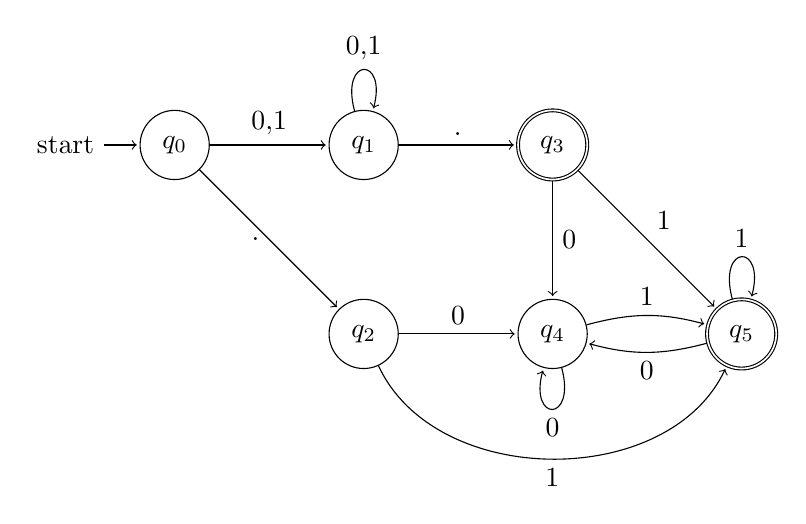
\begin{tikzpicture}[shorten >=1pt,node distance=2.4cm,on grid,auto]
    \node[state,initial] (q0) {$q_0$};
    \node[state] (q1) [right=of q0] {$q_1$};
    \node[state] (q2) [below=of q1] {$q_2$};
    \node[state,accepting] (q3) [right=of q1] {$q_3$};
    \node[state] (q4) [below=of q3] {$q_4$};
    \node[state,accepting] (q5) [right=of q4] {$q_5$};

    \path[->]
    (q0) edge node {0,1} (q1)
         edge node[left] {.} (q2)

    (q1) edge[loop above] node {0,1} ()
         edge node {.} (q3)

    (q2) edge node {0} (q4)
         edge[bend right=65,below] node {1} (q5)

    (q3) edge node {0} (q4)
         edge node {1} (q5)

    (q4) edge[loop below] node {0} ()
         edge[bend left=15] node {1} (q5)

    (q5) edge[bend left=15] node {0} (q4)
         edge[loop above] node {1} ();
\end{tikzpicture}
\]

各状态含义如下：
\begin{itemize}
    \item \(q_0\)：初态，尚未读入任何字符；
    \item \(q_1\)：已读入至少一个二进制数字，但尚未读到小数点；
    \item \(q_2\)：当前只读到一个小数点，前后都为空；
    \item \(q_3\)（接受）：已读到小数点，且点前有数字，点后为空；
    \item \(q_4\)：已进入小数部分，且当前最后一位为 \(0\)；
    \item \(q_5\)（接受）：已进入小数部分，且当前最后一位为 \(1\)；
\end{itemize}

\end{homeworkProblem}

\begin{homeworkProblem}{2.3}

设
\[
A=(Q,\Sigma,\upsilon,q_0,F)
\]
是一个 DFA，\(a\in\Sigma\)，并且对 \(A\) 的所有状态 \(q\in Q\)，都有
\[
\upsilon(q,a)=q.
\]

\begin{enumerate}
    \item 对 \(n\) 进行归纳，证明：对所有 \(n\ge 0\)，都有
    \[
    \tilde{\upsilon}(q,a^n)=q.
    \]
\begin{proof}
    (1)当 \(n=0\) 时，
    \[
    a^0=\varepsilon,
    \]
    由扩展转移函数的定义，
    \[
    \tilde{\upsilon}(q,\varepsilon)=q,
    \]
    因而
    \[
    \tilde{\upsilon}(q,a^0)=q.
    \]

    (2)假设当 \(n=k\) 时结论成立，即
    \[
    \tilde{\upsilon}(q,a^k)=q.
    \]

    则当 \(n=k+1\) 时，
    \[
    \tilde{\upsilon}(q,a^{k+1})
    =
    \tilde{\upsilon}(q,a^k a)
    =
    \upsilon(\tilde{\upsilon}(q,a^k),a).
    \]
    由归纳假设，
    \[
    \upsilon(\tilde{\upsilon}(q,a^k),a)=\upsilon(q,a).
    \]
    再由题设 \(\upsilon(q,a)=q\)，得
    \[
    \tilde{\upsilon}(q,a^{k+1})=q.
    \]

    (3)因此，对所有 \(n\ge 0\)，都有
    \[
    \tilde{\upsilon}(q,a^n)=q.
    \]
    \end{proof}

    \item     证明：\[
    \{a\}^*\subseteq L(A)
    \quad\text{或}\quad
    \{a\}^*\cap L(A)=\varnothing.
    \]
    \begin{proof}
    由第 1 问可知，对任意 \(n\ge 0\)，都有
    \[
    \tilde{\upsilon}(q_0,a^n)=q_0.
    \]
    即从初态 \(q_0\) 出发，读入任意只由 \(a\) 组成的串 \(a^n\) 后，自动机仍停留在初态 \(q_0\)。

    因而，\(\{a\}^*\) 中的串是否被接受，只取决于 \(q_0\) 是否为接受态。

    若 \(q_0\in F\)，则对任意 \(n\ge 0\)，串 \(a^n\) 都被接受，于是
    \[
    \{a\}^*\subseteq L(A).
    \]

    若 \(q_0\notin F\)，则对任意 \(n\ge 0\)，串 \(a^n\) 都不被接受，于是
    \[
    \{a\}^*\cap L(A)=\varnothing.
    \]

    综上，
    \[
    \{a\}^*\subseteq L(A)
    \quad\text{或}\quad
    \{a\}^*\cap L(A)=\varnothing.
    \]
    \end{proof}
\end{enumerate}

\end{homeworkProblem}
    
\begin{homeworkProblem}{2.6}

已知该 \(\varepsilon\)-NFA 的状态集为 \(\{q,p,r\}\)，初态为 \(q\)，终态为 \(\{r\}\)，转移关系如下：
\[
\begin{array}{c|cccc}
 & a & b & c & \varepsilon\\
\hline
\to q & \varnothing & \{q\} & \{p\} & \{r\}\\
p & \{q\} & \{p\} & \{r\} & \varnothing\\
*r & \{p\} & \{r\} & \varnothing & \{q\}
\end{array}
\]

\begin{enumerate}
    
    \item 计算各状态的 \(\varepsilon\) 闭包。

    由于
    \[
    q \xrightarrow{\varepsilon} r,\qquad r \xrightarrow{\varepsilon} q,
    \]
    所以
    \[
    \omega(q)=\{q,r\},\qquad \omega(r)=\{q,r\}.
    \]
    又因为状态 \(p\) 没有 \(\varepsilon\) 转移，所以
    \[
    \omega(p)=\{p\}.
    \]

    因此各状态的 \(\varepsilon\) 闭包为
    \[
    \omega(q)=\{q,r\},\qquad \omega(p)=\{p\},\qquad \omega(r)=\{q,r\}.
    \]

    \item 给出该自动机所接受的长度不大于 \(3\) 的串。

    初态 \(q\) 的 \(\varepsilon\) 闭包为
    \[
    \omega(q)=\{q,r\},
    \]
    记为状态 \(A\)。由于其中包含终态 \(r\)，故 \(A\) 为接受态。

    再记
    \[
    B=\{p\}.
    \]

    由子集构造法可得：
    \[
    A \xrightarrow{a} B,\qquad A \xrightarrow{b} A,\qquad A \xrightarrow{c} B,
    \]
    \[
    B \xrightarrow{a} A,\qquad B \xrightarrow{b} B,\qquad B \xrightarrow{c} A.
    \]

    因此，读入 \(b\) 时状态不变；读入 \(a\) 或 \(c\) 时状态在 \(A,B\) 之间切换一次。
    所以，一个串被接受当且仅当其中 \(a,c\) 的总个数为偶数。

    于是长度不大于 \(3\) 的接受串为：
    \[
    \varepsilon,
    \]
    \[
    b,
    \]
    \[
    aa,\ ac,\ bb,\ ca,\ cc,
    \]
    \[
    aab,\ aba,\ abc,\ acb,\ baa,\ bac,\ bbb,\ bca,\ bcc,\ cab,\ cba,\ cbc,\ ccb.
    \]

    \item 将该自动机转换为 DFA。

    由上面的子集构造法可知，转换后只出现两个状态：
    \[
    A=\{q,r\},\qquad B=\{p\}.
    \]

    其中初态为
    \[
    A=\omega(q)=\{q,r\},
    \]
    接受态为
    \[
    \{A\}=\bigl\{\{q,r\}\bigr\}.
    \]

    其状态转移表为
    \[
    \begin{array}{c|ccc}
     & a & b & c\\
    \hline
    \to *\{q,r\} & \{p\} & \{q,r\} & \{p\}\\
    \{p\} & \{q,r\} & \{p\} & \{q,r\}
    \end{array}
    \]

    因而所求 DFA 为：
    \[
    Q'=\bigl\{\{q,r\},\{p\}\bigr\},\qquad
    \Sigma=\{a,b,c\},
    \]
    \[
    q_0'=\{q,r\},\qquad
    F'=\bigl\{\{q,r\}\bigr\}.
    \]
\end{enumerate}
\end{homeworkProblem}

\begin{homeworkProblem}{2.7}
已知 NFA 的初态为 \(1\)，终态为 \(8\)，其转移关系由题中表给出。

\begin{enumerate}
    \item 计算状态 \(5\) 的 \(\varepsilon\) 闭包。

    由转移表可知：
    \[
    5 \xrightarrow{\varepsilon} \{2,8\},\qquad
    2 \xrightarrow{\varepsilon} \{1\},\qquad
    1 \xrightarrow{\varepsilon} \{2,6\}.
    \]
    因此，从状态 \(5\) 出发，经若干次 \(\varepsilon\) 转移可到达的状态为
    \[
    5,2,8,1,6.
    \]
    所以
    \[
    \omega(5)=\{1,2,5,6,8\}.
    \]

    \item 用自然语言描述该自动机识别的语言。

    由转移关系可知：

    \begin{itemize}
        \item 由
        \[
        1 \xrightarrow{\varepsilon} 6 \xrightarrow{0} 7 \xrightarrow{\varepsilon} 8
        \]
        可知串 \(0\) 被接受；
        \item 由
        \[
        1 \xrightarrow{\varepsilon} 2 \xrightarrow{0} 3 \xrightarrow{\varepsilon} 4 \xrightarrow{1} 5
        \]
        可知串 \(01\) 被接受；
        \item 又因为
        \[
        5 \xrightarrow{\varepsilon} 2,
        \]
        所以可以重复读入若干个 \(01\)；
        \item 并且在若干个 \(01\) 之后，还可以通过
        \[
        2 \xrightarrow{\varepsilon} 1 \xrightarrow{\varepsilon} 6 \xrightarrow{0} 7 \xrightarrow{\varepsilon} 8
        \]
        再接一个 \(0\)。
    \end{itemize}

    因此，该自动机识别的语言是：所有由 \(0\) 和 \(1\) 交替出现、且首符号为 \(0\) 的非空串。


    \item 将该自动机转换为 DFA。

    先求初态 \(1\) 的 \(\varepsilon\) 闭包：
    \[
    \omega(1)=\{1,2,6\}.
    \]
    记
    \[
    A=\{1,2,6\}.
    \]

    从 \(A\) 出发：

    \begin{itemize}
        \item 读入 \(0\) 时，
        \[
        \{1,2,6\}\xrightarrow{0}\{3,7\},
        \]
        再取闭包得
        \[
        \omega(3)\cup\omega(7)=\{3,4\}\cup\{7,8\}=\{3,4,7,8\}.
        \]
        记
        \[
        B=\{3,4,7,8\}.
        \]

        \item 读入 \(1\) 时，无可达状态，因此到
        \[
        D=\varnothing.
        \]
    \end{itemize}

    再看 \(B\) 的转移：

    \begin{itemize}
        \item 读入 \(0\) 时到
        \[
        D=\varnothing;
        \]
        \item 读入 \(1\) 时，先到 \(\{5\}\)，再取闭包得
        \[
        \omega(5)=\{1,2,5,6,8\}.
        \]
        记
        \[
        C=\{1,2,5,6,8\}.
        \]
    \end{itemize}

    再看 \(C\) 的转移：

    \begin{itemize}
        \item 读入 \(0\) 时，先到 \(\{3,7\}\)，再取闭包得
        \[
        B=\{3,4,7,8\};
        \]
        \item 读入 \(1\) 时，到
        \[
        D=\varnothing.
        \]
    \end{itemize}

    对空集状态 \(D\)，有
    \[
    D\xrightarrow{0}D,\qquad D\xrightarrow{1}D.
    \]

    因而转换后的 DFA 状态集合为
    \[
    \{A,B,C,D\}
    \]
    ，其中
    \[
    A=\{1,2,6\},\quad
    B=\{3,4,7,8\},\quad
    C=\{1,2,5,6,8\},\quad
    D=\varnothing.
    \]

    初态为
    \[
    A=\{1,2,6\}.
    \]

    接受态为所有包含 \(8\) 的状态，因此为
    \[
    \{B,C\}.
    \]

    状态转移表为
    \[
    \begin{array}{c|cc}
     & 0 & 1\\
    \hline
    \to A=\{1,2,6\} & B=\{3,4,7,8\} & D=\varnothing\\
    *B=\{3,4,7,8\} & D=\varnothing & C=\{1,2,5,6,8\}\\
    *C=\{1,2,5,6,8\} & B=\{3,4,7,8\} & D=\varnothing\\
    D=\varnothing & D=\varnothing & D=\varnothing
    \end{array}
    \]
\end{enumerate}
\end{homeworkProblem}


\end{document}
